\documentclass{beamer}

\usetheme{Singapore}

\usepackage[utf8]{inputenc}
\usepackage[T1]{fontenc}
\usepackage{textcomp}
\usepackage{amsmath, amssymb, amsthm}
\theoremstyle{plain}
\usepackage{graphicx}
\graphicspath{{./presentation/}}
\usepackage{xcolor}

\newcommand{\pmat}[1]{ \begin{pmatrix}#1\end{pmatrix} }
\newcommand{\seqn}[1]{(#1)^\infty_{n=1}}
\newcommand{\seqk}[1]{(#1)^\infty_{k=1}}
% (series term): returns a series with counter n=1 to \infty.
\newcommand{\infsrsn}[1]{\sum\limits^\infty_{n=1}#1}
\newcommand{\infsrsk}[1]{\sum\limits^\infty_{k=1}#1}
\newcommand{\R}{\mathbb{R}}
\newcommand{\N}{\mathbb{N}}
\newcommand{\Q}{\mathbb{Q}}
\newcommand{\Z}{\mathbb{Z}}
\newcommand{\C}{\mathbb{C}}
\newcommand{\F}{\mathbb{F}}
\newcommand{\cmm}{C(M_1,M_2)}
\newcommand{\met}[1]{\langle M_{#1},\rho_{#1}\rangle}
\newcommand{\ntoinf}{\limits_{n\to\infty}}
\newcommand{\ktoinf}{\limits_{k\to\infty}}
% \newcommand{\onetoinf}[]{^\infty_{n=1}}
\newcommand{\limn}[1]{\lim\ntoinf #1}
\newcommand{\limk}[1]{\lim\ktoinf #1}

\DeclareMathOperator{\spn}{span}
\DeclareMathOperator{\diam}{diam}

\begin{document}

\AtBeginSection[]
{
\begin{frame}<beamer>
\frametitle{Outline}
\tableofcontents[currentsection]
\end{frame}
}


\begin{frame}
  \title{CS2309 Presentation: Constructive Mathematics and Computer Programming}
  \subtitle{Per Martin-Löf 1979}
  \author{Tan Yee Jian}
  \maketitle
\end{frame}
\begin{frame}{Flow}
  \tableofcontents
\end{frame}
\section{Motive}

\subsection{Why constructive mathematics?}
\begin{frame}{Motive - Why constructive mathematics?}
  Imagine the conversation:
  \begin{itemize}
    \pause
    \item You: Is there any integer that is even?
    \pause
    \item Me: Yes there is.
    \pause
    \item You: So, what is it?
    \pause
    \item Me: I can prove that it exists, but I cannot tell you a specific number.
    \pause
    \item You: ???
  \end{itemize}
\end{frame}

\begin{frame}{Motive - Why constructive mathematics?}
 \begin{definition}
   Even numbers are integers $x\in\mathbb{Z}$ where $x\equiv0\mod 2$.
\end{definition}
  \begin{theorem}
    Even numbers exist.
  \end{theorem}
\end{frame}

\begin{frame}{Motive - a non-constructive proof}
  \begin{theorem}
    Even numbers exist.
  \end{theorem}
  \pause
  \begin{proof}[Average constructive proof enjoyer:]
    $0\equiv0\mod 2$. Therefore $0$ is even. Therefore even numbers exist.
  \end{proof}
  \pause
  \begin{proof}[Non-constructive proof:]
    Suppose there are no even numbers. Then for any integer $x\in\mathbb{Z}$, $x\equiv1\mod 2$.
    But by definition of modulo, $2\equiv0\mod2$. Therefore $0=1$, a contradiction.
  \end{proof}
\end{frame}

\begin{frame}{Motive - Why constructive mathematics?}
  Imagine the conversation:
  \begin{itemize}
    \pause
    \item You: Are there two irrational numbers $a, b$, but $a^{b}$ is rational?
    \pause
    \item Me: Yes there is.
    \pause
    \item You: So, what is it?
    \pause
    \item Me: I can prove that it exists, but I don't know any specific $a, b$.
    \pause
    \item You: ???
  \end{itemize}
\end{frame}

\begin{frame}{Motive - another non-constructive proof}
  \begin{theorem}
    There are irrational numbers $a,b$ where $a^{b}$ is rational.
  \end{theorem}
  \pause
  \begin{proof}[Average constructive proof enjoyer:]
    Take $a = \ldots, b = \ldots$, we are done. (??)
  \end{proof}
  \pause
  \begin{proof}[Non-constructive proof:]
    We know $\sqrt{2}$ is irrational. If $\sqrt{2}^{\sqrt{2}}$ is rational, then
    we can let $a=b=\sqrt{2}$. If not, then $a=\sqrt{2}^{\sqrt{2}}, b=\sqrt{2}$,
    we have
    \begin{align*}
      (\sqrt{2}^{\sqrt{2}})^{\sqrt{2}} = \sqrt{2}^{2} = 2
    \end{align*}
    is rational.
  \end{proof}
\end{frame}

\subsection{Type systems}
\begin{frame}{Motive - Types in programming}
\begin{enumerate}
\item High level languages need expressivity with a correctness guarantee - type systems.
        \begin{itemize}
          \item FORTRAN: integers, floats
          \item ALGOL 60: (additionally) boolean
          \item PASCAL: (additionally) enums, tuples, arrays, recursively
                defined types
        \end{itemize}
\pause
\item What does it have to do with constructive mathematics?

(Spoiler) it is constructive, since a valid type is always inhabited by objects,
unlike mathematics, a true proposition is not necessarily inhabited by a witness.
\end{enumerate}
\end{frame}

\section{Related Work}
\begin{frame}{Type Theory and Proof Theory}
  \begin{itemize}
    \item Curry-Howard Isomorphism (``Proposition as Types'')
    \begin{itemize}
      \item (Curry 1934) Intuitionistic Implication Logic
      \item (Curry 1958) Hilbert-styled deduction systems
      \item (Howard 1969) Natural deduction
    \end{itemize}
    \item Martin-Löf's Type Theories: MLTT71, MLTT72, MLTT73, MLTT79
    \item System F (Girard 1972, Reynolds 1974)
  \end{itemize}
\end{frame}

\section{Key Contributions}

\begin{frame}{Key Contributions}
\begin{itemize}
  \item Inductively Typed: There are only 3 initial types.
  \item Popularized the proof-program correspondence.
  \item Influenced the development of interactive theorem provers, best
  popularized when Coq was used to prove the 4-color theorem.
  \item As with most type systems, has very few rules but is very sophisticated.
\end{itemize}
\end{frame}

\section{Results}
\subsection{Intuitionistic Type Theory}
\begin{frame}{Proposition as Types, Proofs as Programs}
  \pause
  \begin{center}
  \begin{tabular}{c|c}
    Mathematics & Programming \\
    \hline
    Proposition
    \pause
                & Type\\
    \pause
    Proof
    \pause
                & Object of a Type\\
    \pause
    Propositions $P, Q$
    \pause
                & Types $P, Q$\\
    \pause
    $P\wedge Q$
    \pause
                & $Tuple(P, Q)$\\
    \pause
    $P\vee Q$
    \pause
                & $Union(P, Q)$\\
    \pause
    $P\implies Q$
    \pause
                & $P \to Q$\\
    \pause
    Proof that $P\implies P$
    \pause
                &   $id:P\to P$\\
    \pause
    $\forall x\in A, B(x)$ & $(f:A \to B(x)): (\prod x:A)B(x)$\\
    \pause
    $\exists x\in A, B(x)$ & $(x: A, y: B(x)): (\sum x:A)B(x)$\\
  \end{tabular}
  \end{center}
\end{frame}

\subsection{Axiom of Choice}
\begin{frame}{Example: Axiom of Choice as a Type}
  \begin{theorem}[Axiom of Choice]
    For any nonempty collection of sets $X$, we have a choice function
    $f:X\to\bigcup X$ such that for any set $Y\in X$, $f(Y)\in Y$.
  \end{theorem}

  \begin{block}{Proof.}
    We write this proposition concretely:
    \begin{align*}
    (\forall x\in A)(\exists {y\in B})y\in x\implies(\exists{f\in A\to B})(\forall{x\in A})f(x) \in x
    \end{align*}
    or rather, as a type: let $A, B, C$ be types.
    \begin{align*}
    (\prod x: A)(\sum {y: B})C(x, y)\to(\sum{f: A\to B})(\prod{x: A})C(x, f(x))
    \end{align*}
  \end{block}
\end{frame}

\begin{frame}{Goal: $(\prod x: A)(\sum {y: B})C(x, y)\to(\sum{f: A\to B})(\prod{x: A})C(x, f(x))$}
    Now all we need to do is to find a term of the type above.

    We start with assuming the LHS is given: let
    \begin{align*}
    &z:(\prod x: A)(\sum {y: B})C(x, y),\text{ and}\\
    &x:A.
    \end{align*}
    Then
    \begin{align}
    z(x): (\sum y\in B)(C(x, y))
    \end{align}
\end{frame}

\begin{frame}{Goal: $(\prod x: A)(\sum {y: B})C(x, y)\to(\sum{f: A\to B})(\prod{x: A})C(x, f(x))$}
  $z(x): (\sum y\in B)(C(x, y))$ can be viewed as a pair, so we can look at its left
  and right entries:
    \begin{align}
    \pi_{1}(z(x))&: B\\
    \pi_{2}(z(x))&:C(x, \pi_{1}(z(x)))
    \end{align}
    Since $x: A$ is arbitrary, we can abstract (2) into a function (a $\Pi$-type),
    then call it, but preserving the type:
    \begin{align}
    (\lambda x:\pi_{1}(z(x)))(x) = \pi_{1}(z(x)): B
    \end{align}
    Substitute (4) into (3), we have the last term $C(x, f(x))$:
    \begin{align}
    \pi_{2}(z(x)):C(x, (\lambda x:\pi_{1}(z(x)))(x))
    \end{align}
\end{frame}

\begin{frame}{Goal: $(\prod x: A)(\sum {y: B})C(x, y)\to(\sum{f: A\to B})(\prod{x: A})C(x, f(x))$}
  We have (5):
  \begin{align*}
    \pi_{2}(z(x)):C(x, (\lambda x:\pi_{1}(z(x)))(x))
  \end{align*}
    Abstract $x$ in (5):
    \begin{align}
    \lambda x:\pi_{2}(z(x)):(\prod x:A)C(x, (\lambda x:\pi_{1}(z(x)))(x))
    \end{align}
    Make a pair (union type):
      \begin{align}
        &(\lambda x: \pi_{1}(z(x)), \lambda x:\pi_{2}(z(x))):\nonumber\\
        &(\sum f:A\to B)(\prod x:A)C(x, (\lambda x:\pi_{1}(z(x)))(x))
      \end{align}
\end{frame}

\begin{frame}{Goal: $(\prod x: A)(\sum {y: B})C(x, y)\to(\sum{f: A\to B})(\prod{x: A})C(x, f(x))$}
      \begin{align*}
        &(\lambda x: \pi_{1}(z(x)), \lambda x:\pi_{2}(z(x))):\nonumber\\
        &(\sum f:A\to B)(\prod x:A)C(x, (\lambda x:\pi_{1}(z(x)))(x))&&(7)
      \end{align*}
    Finally recall $z: LHS$, and we abstract it.
    \begin{align}
    &\lambda z: (\lambda x: \pi_{1}(z(x)), \lambda x:\pi_{2}(z(x))):\nonumber\\
    &(\prod x: A)(\sum {y: B})C(x, y)\to(\sum{f: A\to B})(\prod{x: A})C(x, f(x))
    \end{align}

    The function in (8) has our desired type, therefore it is a proof of the
    ``axiom'' of choice. $\square$
\end{frame}

\section{Discussion}
\begin{frame}{Discussion, Limitation, Future Work}
\begin{itemize}
  \item We have term depend on term: $f(a) = b$, type depend on term
        $x: A, B(x)$, but what about term depend on type? Type depend on Type?
        \pause
  \item Higher-order Type Theories, such as Calculus of Constructions (CoC) is
        commonly used in proof assistants.
        \pause
    \item Two Types are equal if they have exactly the same set of proofs. When
    are two proofs equal? \pause Homotopy Type Theory (Voevodsky 2005).
\end{itemize}
\end{frame}

% \begin{frame}
%   \begin{figure}
%     \centering
% 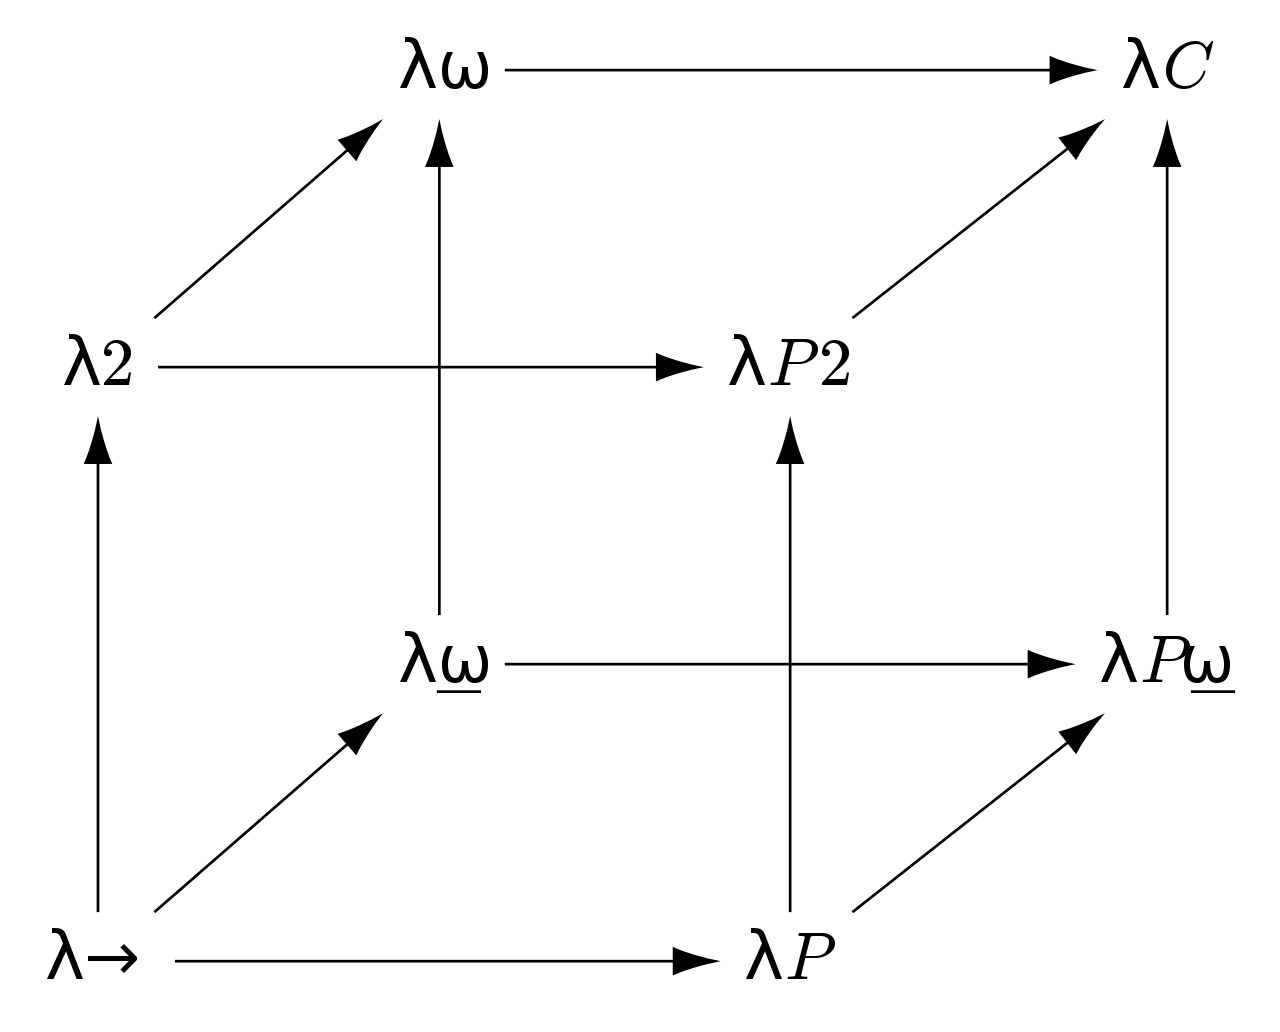
\includegraphics{lambda-cube}
%   \end{figure}
% \end{frame}

\section{Conclusion}
\begin{frame}{Conclusion}
  \begin{figure}
    
\includegraphics{coq} 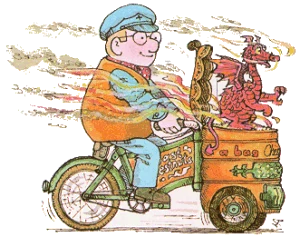
\includegraphics[width=3cm]{idris}
    
\includegraphics[width=3cm]{iris} 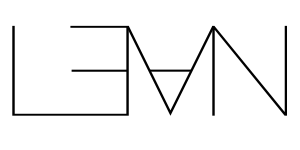
\includegraphics[width=3cm]{lean}
    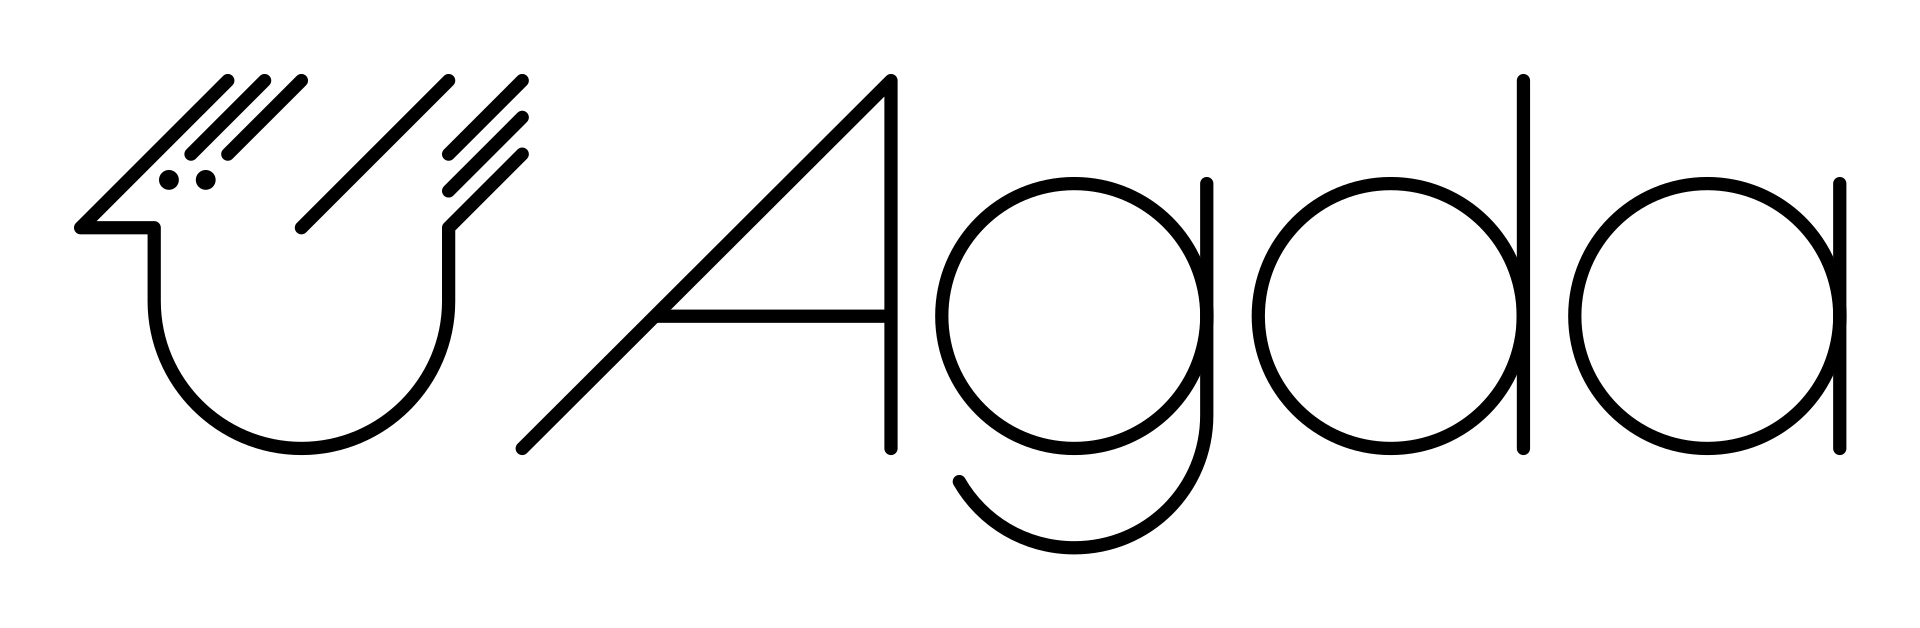
\includegraphics[width=4cm]{agda} \centering
  \end{figure}
\end{frame}
\end{document}
